\documentclass[a4paper,12pt]{article}
% Required packages
\usepackage{amsmath, amsfonts, amssymb, amsthm}
\usepackage{xcolor,graphicx}
\usepackage{fancyhdr} % For header and footer customization
\usepackage{geometry} % To customize page margins
\usepackage{hyperref} % For clickable links
\usepackage{lipsum} % For dummy text generation (optional)
\usepackage{titlesec} % For customizing section and TOC style
\usepackage{helvet}
\usepackage{tcolorbox}
\usepackage{tocloft}
\usepackage{multicol} % For multi-column support
\usepackage{caption} % For adding captions to images and tables
\hypersetup{hidelinks} % Disables colored/boxed links
\usepackage{siunitx} % For proper unit formatting
\usepackage{booktabs} % For professional tables
\usepackage{listings} % For code formatting
\usepackage{booktabs}       % For professional-looking tables

% Define color
\definecolor{blue}{RGB}{31,56,100}

% Set the page margins
\geometry{top=2cm, bottom=2cm, left=2.5cm, right=2cm}
\definecolor{blue}{rgb}{0.2, 0.4, 0.6}

% Set the caption color to light deep blue
% Header and Footer settings
\pagestyle{fancy}
\fancyhf{}
\fancyhead[L]{National Polytechnic Institute of Cambodia}
%\fancyhead[C]{Chapter \thechapter}
\fancyhead[R]{Faculty of Electronic}
\fancyfoot[L]{Power Electronic 2}
\fancyfoot[C]{\thepage}
\fancyfoot[R]{Flyback Converter}
\renewcommand{\headrulewidth}{3pt} % Thin line under the header
\renewcommand{\footrulewidth}{3pt} % Thin line above the footer
%Matlab Code theme
\definecolor{codegreen}{rgb}{0,0.6,0}
\definecolor{codegray}{rgb}{0.5,0.5,0.5}
\definecolor{codepurple}{rgb}{0.58,0,0.82}
\definecolor{backcolour}{rgb}{0.95,0.95,0.92}
\lstdefinestyle{mystyle}{
    backgroundcolor=\color{backcolour},   
    commentstyle=\color{codegreen},
    keywordstyle=\color{blue},
    numberstyle=\tiny\color{codegray},
    stringstyle=\color{codepurple},
    basicstyle=\ttfamily\footnotesize,
    breakatwhitespace=false,         
    breaklines=true,                 
    captionpos=b,                    
    keepspaces=true,                 
    %numbers=left,                    
    %numbersep=5pt,                  
    showspaces=false,                
    showstringspaces=false,
    showtabs=false,                  
    tabsize=2
}
\lstset{style=mystyle}
% Document begins here
\begin{document}

% Title Page
\begin{titlepage}
    \begin{center}
        \begin{minipage}{5cm}
            \begin{flushleft}
                
\includegraphics[scale=0.8,width=3cm]{Pictures/unnamed1.png}
            \end{flushleft}
        \end{minipage}\hfill
        \begin{minipage}{10cm}
            \begin{center}
                \textbf{NATIONAL POLYTECHNIC INSTITUTE OF CAMBODIA }\\[0.5cm]
                \textbf{FACULTY OF ELECTRONIC}\\[0.5cm]
                \textbf{DEPARTMENT OF ELECTRONIC}
            \end{center}
        \end{minipage}\hfill
        \textsc{\Large }\\[1.5cm]
        {\Huge \bfseries Assignment}\\[2cm]
        {\Huge \bfseries Power Electronic 2}
        \textsc{\Large }\\[2.5cm]
        % Title
        \rule{\linewidth}{0.3mm} \\[0.4cm]
        { \huge \bfseries\color{blue} Flyback  Vs Forward Converter\\
        Comparison [ 100W ]\\[0.4cm] }
        \rule{\linewidth}{0.3mm} \\[3cm]
        \begin{flushleft}
            {\large \bfseries Professor's Name : }
            \hspace{6cm}
            {\large \bfseries Meas Saran }\\[1cm]
            {\large \bfseries Student Name : }
            \hspace{6.6cm}
            {\large \bfseries Phon Phearon }\\[0.5cm]
        \end{flushleft}
        % Year
        \vspace{1cm}
        \begin{center}
            {\large \bfseries 2024 - 2025 }
        \end{center}
    \end{center}
\end{titlepage}

% Set Roman page numbering for front matter (cover page and TOC)
\pagenumbering{Roman}

% Table of Contents
\newpage
\tableofcontents
% List of Figure
% \newpage
\listoffigures
\listoftables
\newpage
% Set Arabic page numbering for the content section
\pagenumbering{arabic}
\section{Introduction}
\subsection{Overview of Flyback Converters}
A flyback converter is a kind of isolated switched-mode power supply (SMPS) that isolates its input and output stages electrically by using a transformer. Modern power electronics are built on this isolation, which guarantees safety and adherence to legal requirements. The ability of flyback converters to offer several regulated output voltages, their affordability, and their small size have made them well-known and solidified their place in a variety of applications, from industrial systems to consumer electronics. In applications where efficiency and space are crucial, such as LED drivers, phone chargers, and television auxiliary power sources, they are essential.\\[0.3cm]
The significance of flyback converters has increased in today's technologically advanced world due to the rising need for dependable, lightweight, and energy-efficient power solutions. Because of their straightforward design and ability to function in both continuous conduction mode (CCM) and discontinuous mode (DCM), engineers may customize them to meet a range of power needs.
\begin{multicols}{2}  % Start two-column layout
    % First column: image 1
    \noindent
    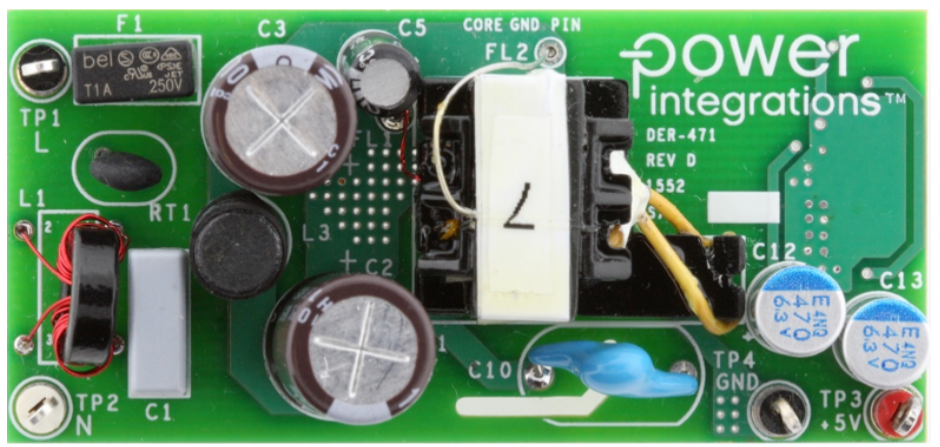
\includegraphics[width=1\linewidth]{Pictures/pics/1.png}
    \captionof{figure}{\textcolor{blue}{\textit{\footnotesize15-W Isolated Flyback Converter}}}
    \hfill
    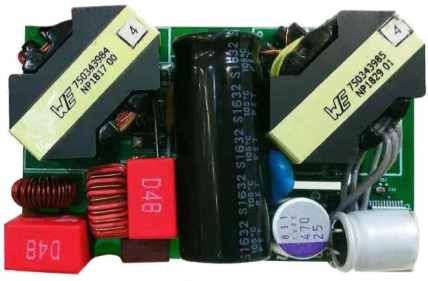
\includegraphics[width=0.8\linewidth]{Pictures/pics/2.png}
    \captionof{figure}{\textcolor{blue}{\textit{\footnotesize 100-W AC/DC adapter}}}
\end{multicols}
\subsection{Purpose of the Report}
% \noindent % To make sure the text starts immediately after the multicolumn environment ends
\noindent The purpose of this report is to provide a comprehensive analysis of flyback converters, focusing on their working principle, key design considerations, and practical applications. By exploring these aspects, the report aims to highlight the technical nuances that make flyback converters indispensable in modern electronics while addressing challenges such as leakage inductance, switching losses, and electromagnetic interference (EMI).

% % Now switching to single-column layout for the next figure and caption
\begin{figure}[h!]
    \centering
    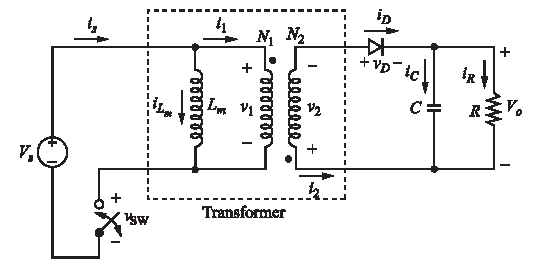
\includegraphics[width=0.6\linewidth]{Pictures/pics/6.pdf}
    \caption{\textcolor{blue}{\textit{\footnotesize Equivalent circuit using a transformer model that includes the magnetizing inductance}}}
\end{figure}
\newpage
\section{Fundatmental Of Flyback Converter}
\subsection{Basic Operating Principles}
\subsubsection*{Energy Storage in the Transformer During the ON Phase}
\begin{itemize}
    \item Explain that during the ON phase , when the switch (usually a MOSFET) is closed, current flows through the primary winding of the transformer.
    \item This current builds up a magnetic field in the transformer core, storing energy in the form of magnetic flux.
    \item The secondary winding is isolated during this phase, and no current flows to the output.
\end{itemize}
\begin{figure}[h!]
    \centering
    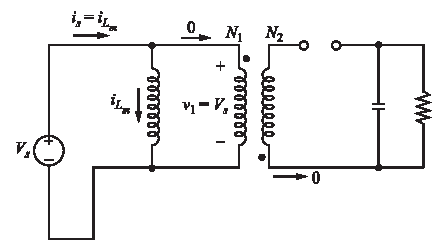
\includegraphics[width=0.6\linewidth]{Pictures/pics/4.pdf}
    \caption{\textcolor{blue}{\textit{\footnotesize  Circuit for the switch on.}}}
\end{figure}
\subsubsection*{Energy Transfer to the Output During the OFF Phase}
\begin{itemize}
    \item When the switch is turned OFF , the magnetic field collapses, inducing a voltage across the secondary winding.
    \item This voltage forward-biases the diode on the secondary side, allowing current to flow through the load and charge the output capacitor.
    \item The energy stored in the transformer is transferred to the output during this phase.
\end{itemize}
\begin{figure}[h!]
    \centering
    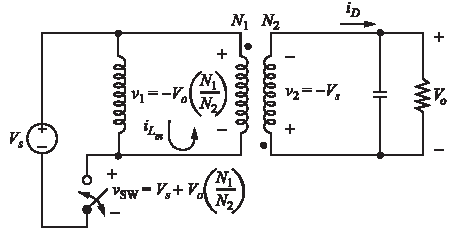
\includegraphics[width=0.6\linewidth]{Pictures/pics/5.pdf}
    \caption{\textcolor{blue}{\textit{\footnotesize   Circuit for the switch off.}}}
\end{figure}
\subsection{Key Components}
\begin{enumerate}
    \item \textbf{Transformer}: Stores energy during the ON phase and transfers it to the output during the OFF phase. Also provides voltage transformation and isolation.
    \item \textbf{Switch (MOSFET/IGBT)}: Controls the flow of current through the primary winding by turning ON and OFF.
    \item  \textbf{Diode (Output Rectifier)}: Rectifies the AC waveform from the secondary winding into DC.
    \item \textbf{Output Capacitor}:  Smooths the rectified output voltage and reduces ripple.
    \item \textbf{Input Capacitor}: smooths the input voltage and reduces ripple caused by pulsating current.
\end{enumerate}
\subsection{Modes of Operation}
\subsubsection*{Continuous Conduction Mode (CCM)}
\begin{itemize}
    \item In CCM, the current in the transformer never fully drops to zero during the OFF phase.
    \item This mode is typically used in higher-power applications because it reduces ripple current and improves efficiency.
    \item However, it requires more complex control and larger magnetics.
\end{itemize}
\subsubsection*{Discontinuous Conduction Mode (DCM)}
\begin{itemize}
    \item In DCM, the current in the transformer drops to zero before the next switching cycle begins.
    \item This mode is simpler to control and is often used in low-power applications.
    \item However, it can lead to higher peak currents and more EMI.
\end{itemize}
\subsubsection*{Boundary Conduction Mode (BCM)}
\begin{itemize}
    \item BCM operates at the boundary between CCM and DCM, where the current just reaches zero at the end of the OFF phase.
    \item This mode offers a balance between efficiency and simplicity, making it popular in medium-power applications.
\end{itemize}

\section{Mathematical Modeling}
\subsection{Derivation of the Voltage Conversion Equation}
\subsubsection*{Energy Stored During the ON Phase}
During the ON phase, the current in the primary winding increases linearly due to the applied input voltage ($V_{in}$). The rate of change of current is given by:
\[
\frac{dI_p}{dt} = \frac{V_{in}}{L_p}
\]
where:
\begin{itemize}
    \item $I_p$: Primary winding current.
    \item $L_p$: Inductance of the primary winding.
\end{itemize}

The total energy stored in the primary winding during the ON phase is:
\[
E_{stored} = \frac{1}{2} L_p I_p^2
\]

The peak primary current ($I_p$) at the end of the ON phase can be expressed as:
\[
I_p = \frac{V_{in} \cdot D \cdot T_s}{L_p}
\]
where:
\begin{itemize}
    \item $D$: Duty cycle (fraction of time the switch is ON).
    \item $T_s$: Switching period ($T_s = 1/f_s$, where $f_s$ is the switching frequency).
\end{itemize}

Substituting $I_p$ into the energy equation:
\[
E_{stored} = \frac{1}{2} L_p \left(\frac{V_{in} \cdot D \cdot T_s}{L_p}\right)^2
\]
\[
E_{stored} = \frac{1}{2} \cdot \frac{(V_{in} \cdot D \cdot T_s)^2}{L_p}
\]

\subsubsection*{Energy Transferred During the OFF Phase}
During the OFF phase, the energy stored in the transformer is transferred to the load. The output power ($P_{out}$) is related to the energy transferred per switching cycle:
\[
P_{out} = \frac{E_{transferred}}{T_s}
\]

Since the energy stored in the transformer is equal to the energy transferred to the load in steady-state:
\[
E_{transferred} = E_{stored}
\]

Thus:
\[
P_{out} = \frac{E_{stored}}{T_s}
\]

Substitute $E_{stored}$:
\[
P_{out} = \frac{1}{2} \cdot \frac{(V_{in} \cdot D \cdot T_s)^2}{L_p \cdot T_s}
\]
\[
P_{out} = \frac{1}{2} \cdot \frac{V_{in}^2 \cdot D^2 \cdot T_s}{L_p}
\]

\subsubsection*{Relating Output Voltage to Input Voltage}
The output power ($P_{out}$) is also given by:
\[
P_{out} = V_{out} \cdot I_{out}
\]

Assuming the output current ($I_{out}$) is constant and related to the duty cycle, we can express the relationship between the input and output voltages using the transformer turns ratio ($N_s/N_p$).

From the transformer equations:
\[
\frac{V_{out}}{V_{in}} = \frac{N_s}{N_p} \cdot D
\]

Rearranging:
\[
V_{out} = \frac{N_s}{N_p} \cdot D \cdot V_{in}
\]
\subsection{Power Stage Calculation Formulas}
\subsubsection*{1. Duty Cycle ($D$)}
$$
D = \frac{\frac{V_{out}}{V_{in}}}{\frac{N_s}{N_p} + \frac{V_{out}}{V_{in}}}
$$
The duty cycle determines the fraction of time the switch is ON during a switching cycle. It depends on the input/output voltages and the transformer turns ratio.

\subsubsection*{2. Load Resistance ($R_{load}$)}
$$
R_{load} = \frac{V_{out}}{I_{out}}
$$
The load resistance is calculated from the output voltage and current. It represents the effective resistance seen by the converter.

\subsubsection*{3. Output Current ($I_{out}$)}
$$
I_{out} = \frac{P_{out}}{V_{out}}
$$
The output current is derived from the output power and voltage. It indicates the current supplied to the load.

\subsubsection*{4. Ripple Current ($\Delta I_L$)}
$$
\Delta I_L = 0.3 \cdot I_{in}, \quad I_{in} = \frac{P_{out}}{V_{in}}
$$
The ripple current is typically chosen as 30\% of the average input current. It ensures stable operation in Continuous Conduction Mode (CCM).

\subsubsection*{5. Ripple Voltage ($\Delta V_{out}$)}
$$
\Delta V_{out} = 0.01 \cdot V_{out}
$$
The ripple voltage is assumed to be 1\% of the output voltage. It represents the allowable voltage fluctuation at the output.

\subsubsection*{6. Magnetizing Inductance ($L_m$)}
$$
L_m = \frac{V_{in} \cdot D}{f_{sw} \cdot \Delta I_L}
$$
The magnetizing inductance determines the energy stored in the transformer during the ON time of the switch.

\subsubsection*{7. Primary Inductance ($L_p$)}
$$
L_p = L_m
$$
The primary inductance is equal to the magnetizing inductance.

\subsubsection*{8. Secondary Inductance ($L_s$)}
$$
L_s = L_p \cdot \left(\frac{N_s}{N_p}\right)^2
$$
The secondary inductance is scaled by the square of the transformer turns ratio.

\subsubsection*{9. Magnetizing Inductor Ripple Current}
- Maximum Current:
$$
I_{max} = I_{in} + \frac{\Delta I_L}{2}
$$
- Minimum Current:
$$
I_{min} = I_{in} - \frac{\Delta I_L}{2}
$$
- Average Current:
$$
I_{avg} = I_{in}
$$
These values represent the peak, minimum, and average currents in the magnetizing inductor.
\newpage
\subsection{CCM and DCM Waveform}
\begin{multicols}{2}  % Start two-column layout
    % First column: image 1
    \noindent
    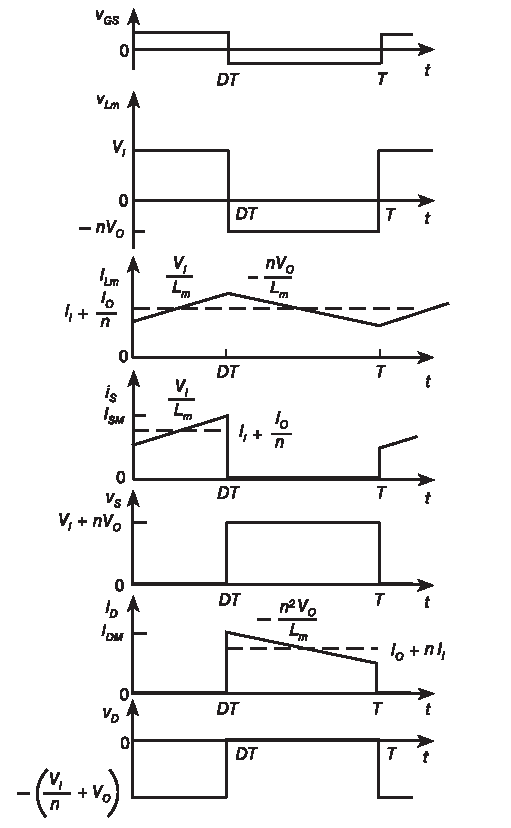
\includegraphics[width=1.07\linewidth]{Pictures/pics/7.pdf}
    \captionof{figure}{\textcolor{blue}{\textit{\footnotesize Idealized current and voltage waveforms in the PWM inverting flyback converter for CCM.}}}
    \hfill
    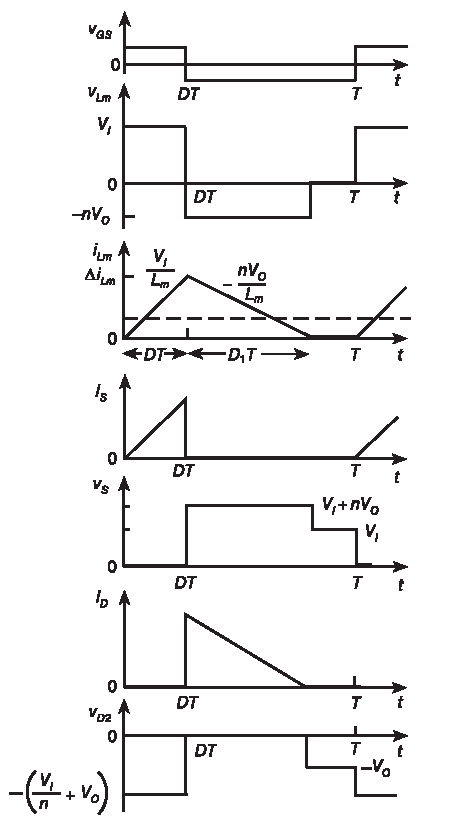
\includegraphics[width=1\linewidth]{Pictures/pics/8.pdf}
    \captionof{figure}{\textcolor{blue}{\textit{\footnotesize Idealized current and voltage waveforms in the PWM flyback converter for DCM}}}
\end{multicols}
\section{Design and Implementation}
\subsection{Power Stage Calculation and Component Selection}
Design of a 120W flyback Converter Operating in Continuous Conduction Mode (CCM) with
the following specifications:
\newpage
\begin{table}[h!]
    \centering
    \begin{tabular}{l l l}
        \toprule
        \textbf{Parameter} & \textbf{Symbol} & \textbf{Value} \\
        \midrule
        Input Voltage & $ V_{in} $ & 310 V \\
        Output Voltage & $ V_{out} $ & 24 V \\
        Output Power & $ P_{out} $ & 100 W \\
        Switching Frequency & $ f_{sw} $ & 100 kHz \\
        Diode Voltage & $ V_d $ & 1 V \\
        Ripple Current Rate & - & 30\% \\
        Ripple Voltage Rate & - & 1\% \\
        Duty Cycle & $ D $ & 30\%\\
        efficiency & $ \eta $ & 90\%\\
        \bottomrule
    \end{tabular}
    \caption{Input Parameters}
\end{table}
\subsection{Power Stage Calculations}
\subsubsection*{1. Transformer Turn Ratio}
\[
\frac{N_p}{N_s} = \frac{V_{in} \cdot D}{(V_{out} + V_f)(1 - D)} 
= \frac{310 \cdot 0.3}{(24 + 1) \cdot 0.7} \approx \boxed{5.314:1}
\]
\subsubsection*{2. Output Current}
\[
I_{out} = \frac{P_{out}}{V_{out}} = \frac{100}{24} \approx \boxed{4.167\,\text{A}}
\]
\subsection*{3. Load Resistance}
\[
R_{\text{load}} = \frac{V_{out}}{I_{out}} = \frac{24}{4.167} \approx \boxed{5.76\,\Omega}
\]
\subsection*{$\bullet$ Transformer Primary Side Calculation}
\subsubsection*{4. Primary Average Current}
\[
I_{\text{primary\_avg}} = \frac{P_{in}}{V_{in} \cdot D} 
= \frac{111.11}{310 \cdot 0.3} \approx \boxed{1.195\,\text{A}}
\]
\subsubsection*{5. Primary Ripple Current}
\[
\Delta I_{L1} = 0.3 \cdot I_{\text{primary\_avg}} = 0.3 \cdot 1.195 \approx \boxed{0.358\,\text{A (p-p)}}
\]
\subsubsection*{6. Primary Maximum Current}
\[
I_{\text{primary\_max}} = I_{\text{primary\_avg}} + \frac{\Delta I_{L1}}{2} 
\approx 1.195 + 0.179 \approx \boxed{1.374\,\text{A}} 
\]
\subsubsection*{7. Primary Minimum Current}
\[
I_{\text{primary\_min}} = I_{\text{primary\_avg}} - \frac{\Delta I_{L1}}{2} 
\approx 1.195 - 0.179 \approx \boxed{1.016\,\text{A}} \\
\]
\subsubsection*{8. Primary rms Current}
\[
I_{\text{primary\_rms}} = \sqrt{\frac{1}{3} \left( I_{\text{primary\_peak}}^2 + I_{\text{primary\_peak}}I_{\text{primary\_min}} + I_{\text{primary\_min}}^2 \right)} 
\approx \boxed{1.21\,\text{A}}
\]
\subsubsection*{9. Magnetizing Inductance or Primary Inductance}
\[
L_p = \frac{V_{in} \cdot D}{\Delta I_{L1} \cdot f_{sw}} 
= \frac{310 \cdot 0.3}{0.358 \cdot 100 \cdot 10^3} \approx \boxed{2.595\,\text{mH}}
\]
\subsection*{$\bullet$ Transformer Secondary Side Calculation}
\subsubsection*{10. Secondary Average Current}
\[
I_{\text{secondary\_avg}} = I_{out} = \boxed{4.167\,\text{A}}
\]
\subsubsection*{11. Secondary Ripple Current}
\[
\Delta I_{\text{secondary}} = \Delta I_{L1} \cdot I_{\text{secondary\_avg}} =0.358 \cdot 5.314 = \boxed{1.9332}
\]
\subsubsection*{12. Secondary Maximum Current }
\[
I_{\text{secondary\_max}} = I_{\text{primary\_max}} \cdot \frac{N_p}{N_s} 
\approx 1.374 \cdot 5.314 \approx \boxed{7.30\,\text{A}} \\
\]
\subsubsection*{13. Secondary Minimum Current}
\[
I_{\text{secondary\_min}} = I_{\text{secondary\_peak}} - \Delta I_{\text{secondary}} \\
= 7.30 - (0.358 \cdot 5.314) \approx \boxed{5.40\,\text{A}} \\
\]
\subsubsection*{14. Secondary rms Current}
\[
I_{\text{secondary\_rms}} = \sqrt{\frac{1}{3} \left( I_{\text{secondary\_max}}^2 + I_{\text{secondary\_max}}I_{\text{secondary\_min}} + I_{\text{secondary\_min}}^2 \right) \cdot (1 - D)} 
\approx \boxed{5.33\,\text{A}}
\]
\subsubsection*{15. Secondary Inductance}
\[
L_s = L_p \cdot \left( \frac{N_s}{N_p} \right)^2 
= 2.595 \cdot \left( \frac{1}{5.314} \right)^2 \approx \boxed{91.7\,\mu\text{H}}
\]
\subsection*{$\bullet$ Output Capacitor}
\subsubsection*{16. Ripple Output Voltage}
\[
\Delta V_{ripple} = 0.1 \cdot V_{out} = 0.1 \cdot 24 = \boxed{0.24V}
\]
\subsubsection*{17. Output Capacitor}
\[
C = \frac{I_{out} \cdot D}{f_{sw} \cdot \Delta V_{\text{ripple}}} 
= \frac{4.167 \cdot 0.3}{100 \cdot 10^3 \cdot 0.24} \approx \boxed{52.09\,\mu\text{F}}
\]
\subsection*{$\bullet$ Component Selection}
\subsubsection*{18. MOSFET}
\begin{center}
    \begin{minipage}{0.4\textwidth}
        \centering
        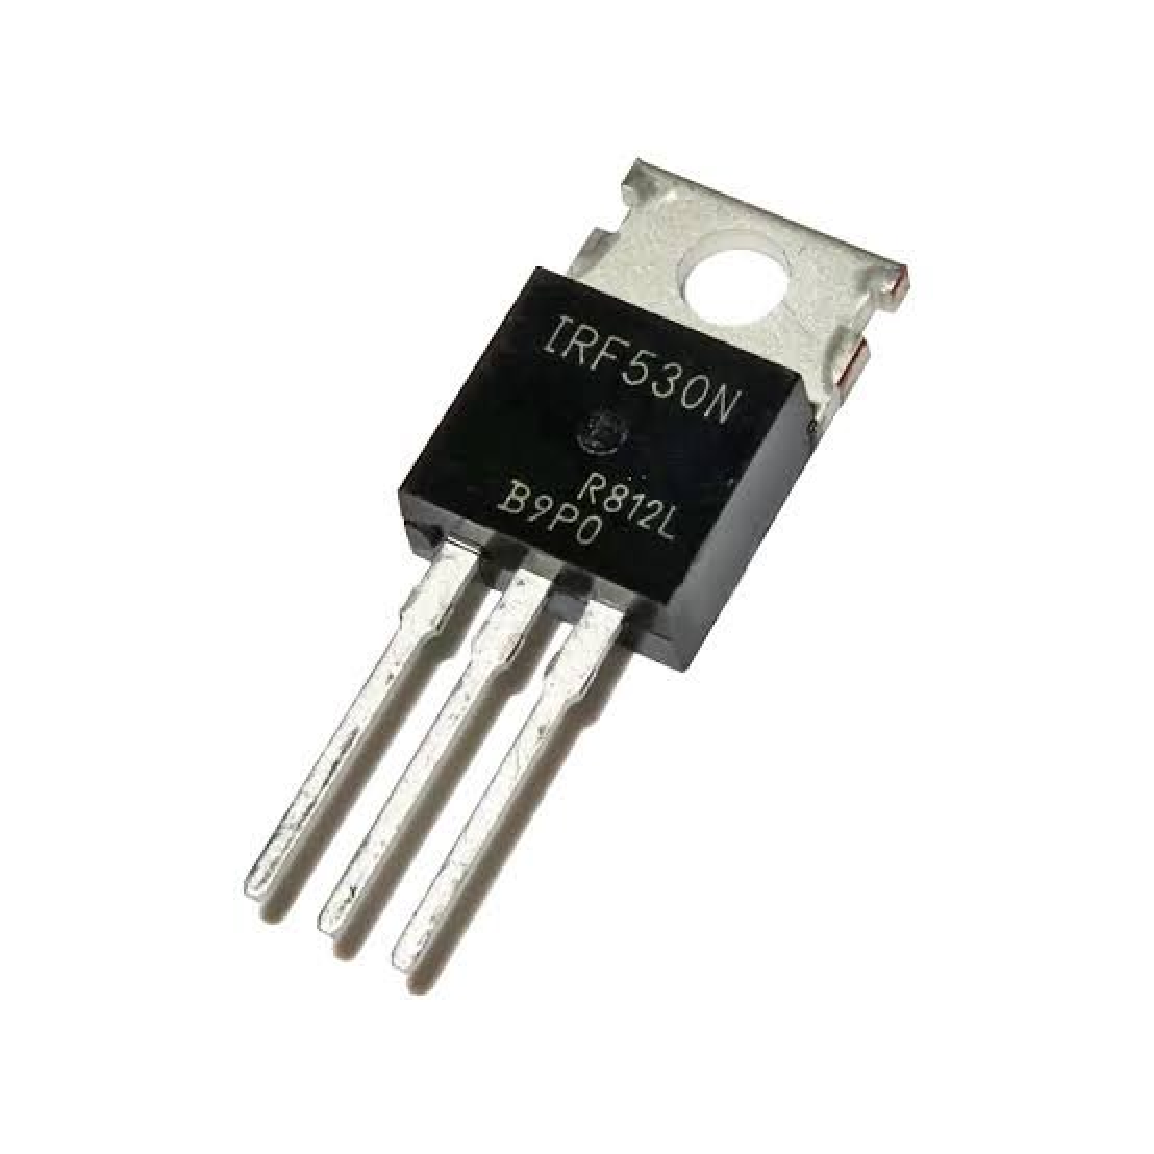
\includegraphics[width=0.8\linewidth]{Pictures/pics/mosfet.pdf} % Replace with your image file
        %\captionof{figure}{This is a figure.} % Add a caption
    \end{minipage}
    \hfill % Adds space between the minipages
    \begin{minipage}{0.55\textwidth}
    \centering
    \captionof{table}{IRF540N MOSFET}
    \label{tab:IRF530}
    \begin{tabular}{lcc}
    \toprule
    \footnotesize
    \textbf{Parameter} & \textbf{Value} & \textbf{Test Conditions} \\
    \midrule
     $V_{DS}$ & \SI{100}{\volt} & Absolute Maximum Rating \\
     $I_D$ & \SI{14}{\ampere} & $T_C = \SI{25}{\celsius}$ \\
     & \SI{10}{\ampere} & $T_C = \SI{100}{\celsius}$ \\
     $R_{DS(on)}$ & \SI{0.16}{\ohm} & $V_{GS} = \SI{10}{\volt}, I_D = \SI{8.4}{\ampere}$ \\
    \bottomrule
    \end{tabular}
    \end{minipage}
\end{center}
\subsubsection*{19. Diode Selection}
\begin{center}
    \begin{minipage}{0.4\textwidth}
        \centering
        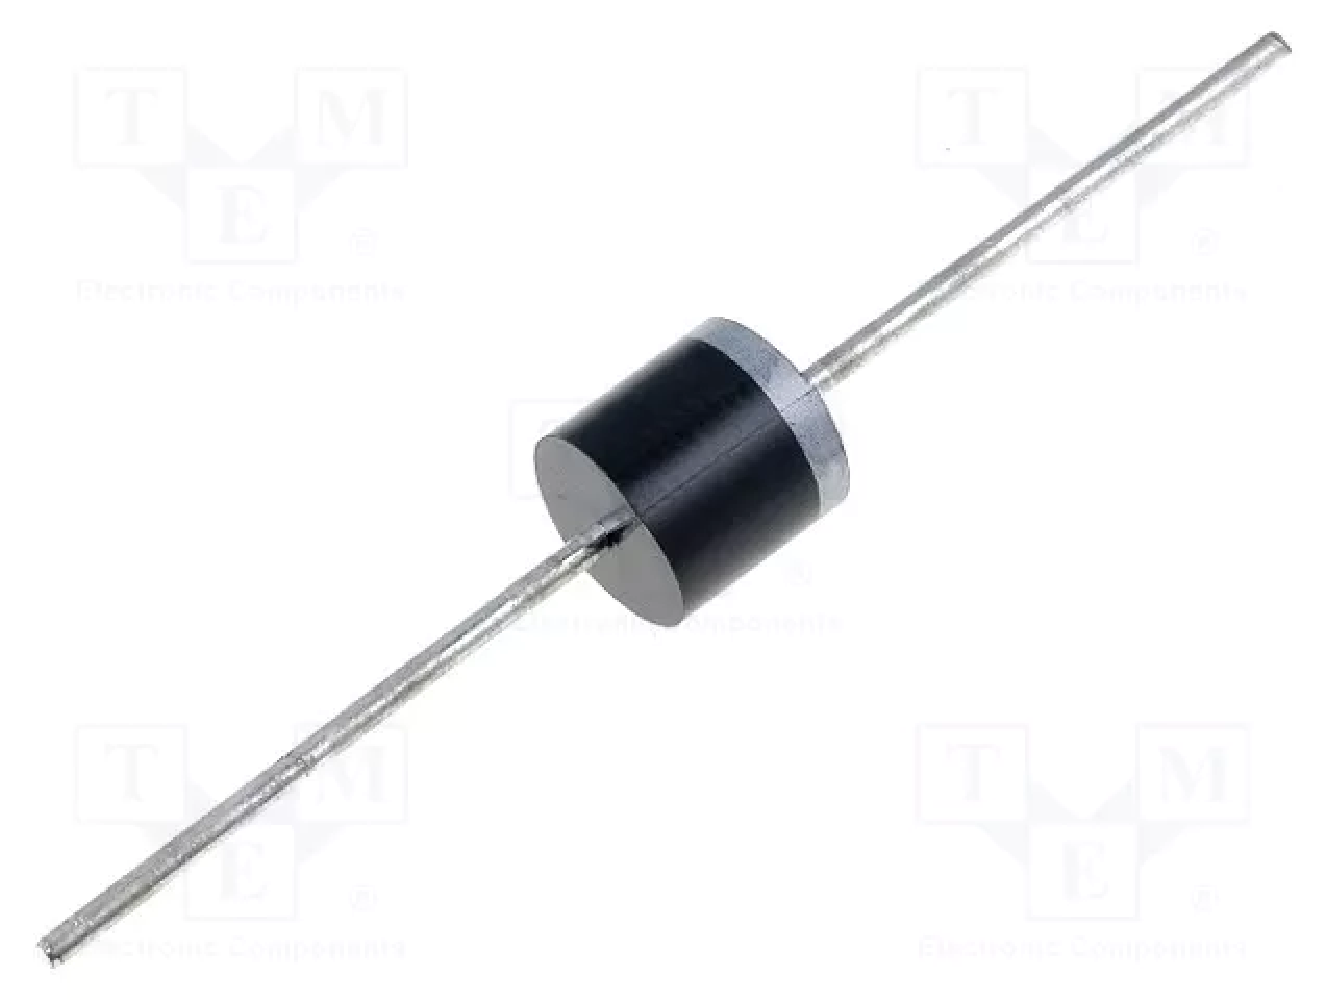
\includegraphics[width=0.7\linewidth]{Pictures/pics/diode.pdf} % Replace with your image file
        %\captionof{figure}{This is a figure.} % Add a caption
    \end{minipage}
    \hfill % Adds space between the minipages
    \begin{minipage}{0.55\textwidth}
    \centering
    \captionof{table}{15SQ045 Schottky Diode}
        \label{tab:SR510}
        \begin{tabular}{lcc}
        \toprule
        \textbf{Parameter} & \textbf{Value} & \textbf{Test Conditions} \\
        \midrule
        $V_{RRM}$ & \SI{100}{\volt} & Maximum repetitive rating \\
        $I_F$ & \SI{5}{\ampere} & Continuous, $T_A = \SI{25}{\celsius}$ \\
        \bottomrule
        \end{tabular}
    \end{minipage}
\end{center}
\subsection*{$\bullet$ Transformer Design}
\begin{table}[h!]
 \caption{Input Parameters for Flyback Transformer Design}
    \label{tab:input_parameters}
    \centering
    \begin{tabular}{l l l}
    \toprule
    \textbf{Parameter} & \textbf{Value} & \textbf{Unit} \\
    \midrule
    Inductance ($L$) & $\SI{2.955e-3}{}$ & \si{\henry} \\
    Primary Peak Current ($I_{p,\text{pk}}$) & $\SI{1.374}{}$ & \si{\ampere} \\
    Output Power ($P_o$) & $\SI{100}{}$ & \si{\watt} \\
    Ferrite Core Flux Density ($B_m$) & $\SI{0.25}{}$ & \si{\tesla} \\
    Regulation ($\alpha$) & $1$ & - \\
    Diode Drop Voltage ($V_d$) & $\SI{1}{}$ & \si{\volt} \\
    Duty Cycle ($D$) & $0.3$ & - \\
    Dwell Time Ratio ($D_w$) & $0.1$ & - \\
    Window Utilization ($K_u$) & $0.4$ & - \\
    Switching Frequency ($F$) & $\SI{100e3}{}$ & \si{\hertz} \\
    \bottomrule
    \end{tabular}
\end{table}
\subsubsection*{Energy-Handling Capability ($E$)}
\[
E = \frac{L \cdot I_{p,\text{pk}}^2}{2} = \frac{(2.955 \times 10^{-3}) \cdot (1.374)^2}{2} = \frac{(2.955 \times 10^{-3}) \cdot 1.887}{2} \approx \SI{0.00278}{\watt\second}
\]
\subsubsection*{Electrical Condition ($K_e$)}
\[
K_e = 0.145 \cdot P_o \cdot B_m^2 \cdot 10^{-4} = 0.145 \cdot 100 \cdot (0.25)^2 \cdot 10^{-4} = 9.0625 \times 10^{-5}
\]
\subsubsection*{Core Geometry ($K_g$)}
\[
K_g = \frac{E^2}{K_e \cdot \alpha} = \frac{(0.00278)^2}{9.0625 \times 10^{-5}} = \frac{7.7284 \times 10^{-6}}{9.0625 \times 10^{-5}} \approx 0.0853
\]
\begin{figure}[h!]
    \centering
    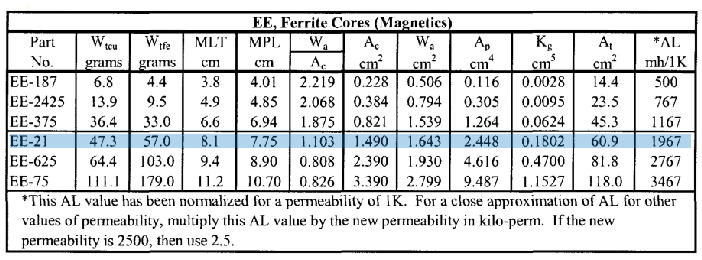
\includegraphics[width=1\linewidth]{Pictures/pics/EE21_selected.pdf}
    \caption{\textcolor{blue}{\textit{\footnotesize PQ Core Parameter Table List}}}
\end{figure} 
\begin{figure}[h!]
    \centering
    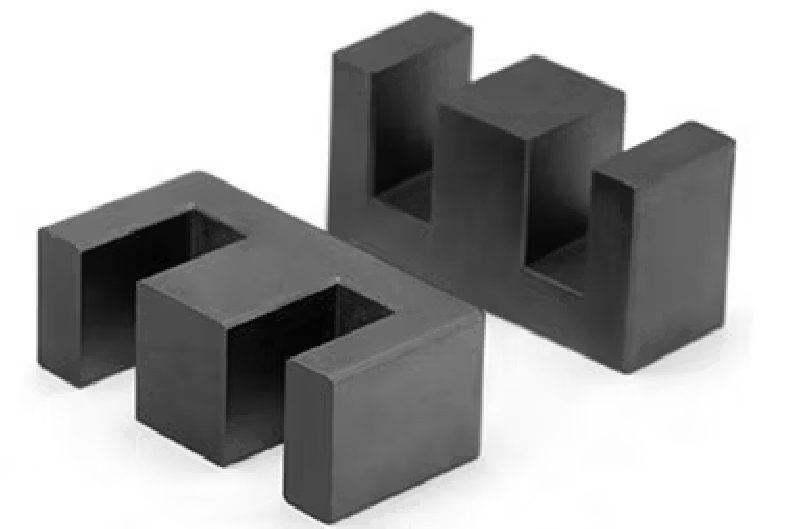
\includegraphics[width=0.5\linewidth]{Pictures/pics/eecore.pdf}
    \caption{\textcolor{blue}{\textit{\footnotesize EE21 Core}}}
\end{figure} 
\begin{table}[h!]
\centering
\begin{tabular}{l l l}
\toprule
\textbf{Parameter} & \textbf{Value} & \textbf{Unit} \\
\midrule
Magnetic Path Length ($MPL$) & $\SI{7.75}{}$ & \si{\centi\meter} \\
Core Weight ($W_{\text{core}}$) & $\SI{57}{}$ & \si{\gram} \\
Copper Weight ($W_{\text{copper}}$) & $\SI{47.3}{}$ & \si{\gram} \\
Mean Length Turn ($MLT$) & $\SI{8.1}{}$ & \si{\centi\meter} \\
Cross-Sectional Area ($A_c$) & $\SI{1.490}{}$ & \si{\centi\meter\squared} \\
Window Area ($W_a$) & $\SI{1.643}{}$ & \si{\centi\meter\squared} \\
Core Product ($A_p$) & $\SI{2.448}{}$ & \si{\centi\meter\tothe{4}} \\
Core Geometry ($Kg_s$) & $\SI{0.1802}{}$ & \si{\centi\meter\tothe{5}} \\
\bottomrule
\end{tabular}
\caption{Selected Core Parameters for Transformer Design}
\label{tab:core_parameters}
\end{table}
\subsubsection*{Current Density ($J$)}
\[
J = \frac{2 \cdot E \cdot 10^4}{B_m \cdot A_p \cdot K_u} = \frac{2 \cdot 0.00278 \cdot 10^4}{0.25 \cdot 2.448 \cdot 0.4} \approx \SI{227.1}{\ampere\per\centi\meter\squared}
\]
\subsubsection*{Primary Wire Area ($A_{pw}$)}
\[
A_{pw} = \frac{I_{p,\text{rms}}}{J} = \frac{1.21}{227.1} \approx \SI{0.00428}{\centi\meter\squared}
\]
\subsubsection*{Number of Primary Turns ($N_p$)}
\[
N_p = \frac{K_u \cdot W_a / 2}{3 \cdot A_{ws}} = \frac{0.4 \cdot (1.643 / 2)}{3 \cdot 0.01} \approx 11
\]
\subsubsection*{Secondary Wire Area ($A_{sw}$)}
\[
A_{sw} = \frac{I_{s,\text{rms}}}{J} = \frac{5.33}{227.1} \approx \SI{0.0227}{\centi\meter\squared}
\]
\subsubsection*{Secondary Turns ($N_s$)}
\[
N_s = \frac{N_p \cdot (V_o + V_d) \cdot (1 - D - D_w)}{V_i \cdot D} = \frac{11 \cdot (24 + 1) \cdot (1 - 0.3 - 0.1)}{310 \cdot 0.3} \approx 2
\]
\subsubsection*{Gap Length ($L_g$)}
\[
L_g = \left| \frac{0.4 \cdot \pi \cdot N_p^2 \cdot A_c \cdot 10^{-8}}{L} - \frac{MPL}{\mu_0} \right| = \left| \frac{0.4 \cdot \pi \cdot 11^2 \cdot 1.490 \cdot 10^{-8}}{2.955 \times 10^{-3}} - \frac{7.75}{2500} \right| \approx \SI{0.00453}{\centi\meter}
\]
\subsection{Flyback Convert Simulation}
\begin{figure}[h!]
    \centering
    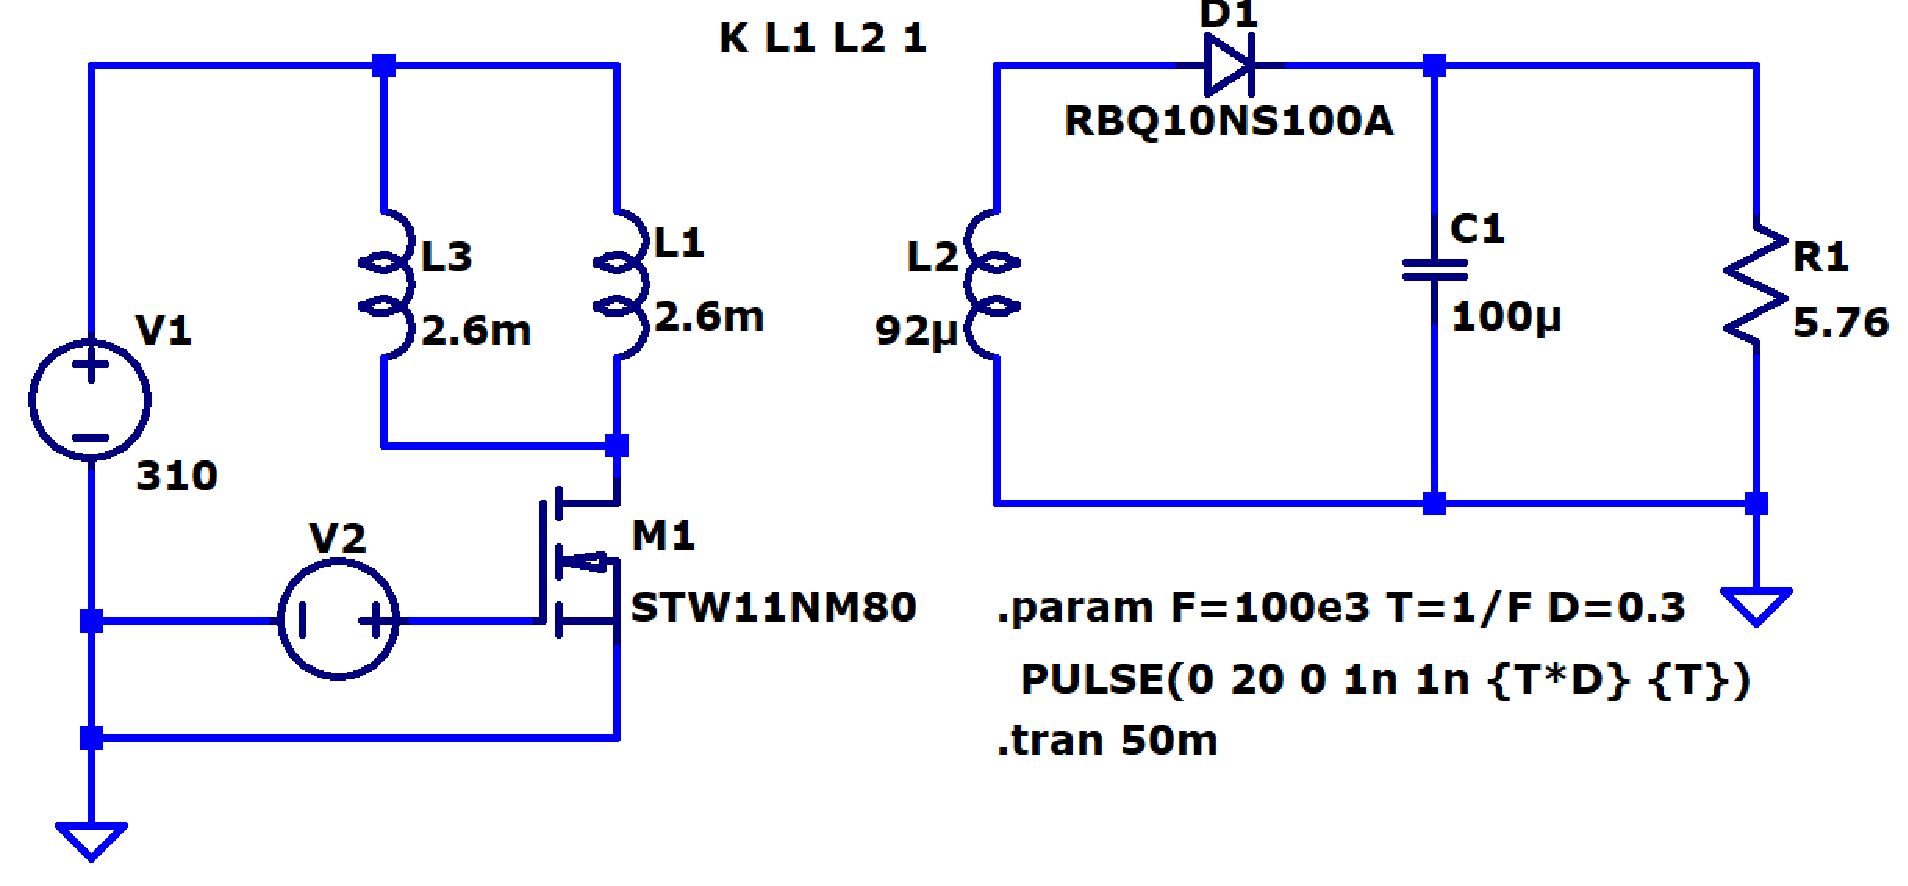
\includegraphics[width=0.8\linewidth]{Pictures/pics/LT_schem.pdf}
    \caption{\textcolor{blue}{\textit{\footnotesize Flyback Converter Schematic on LTspice}}}
\end{figure}
\begin{figure}[h!]
    \centering
    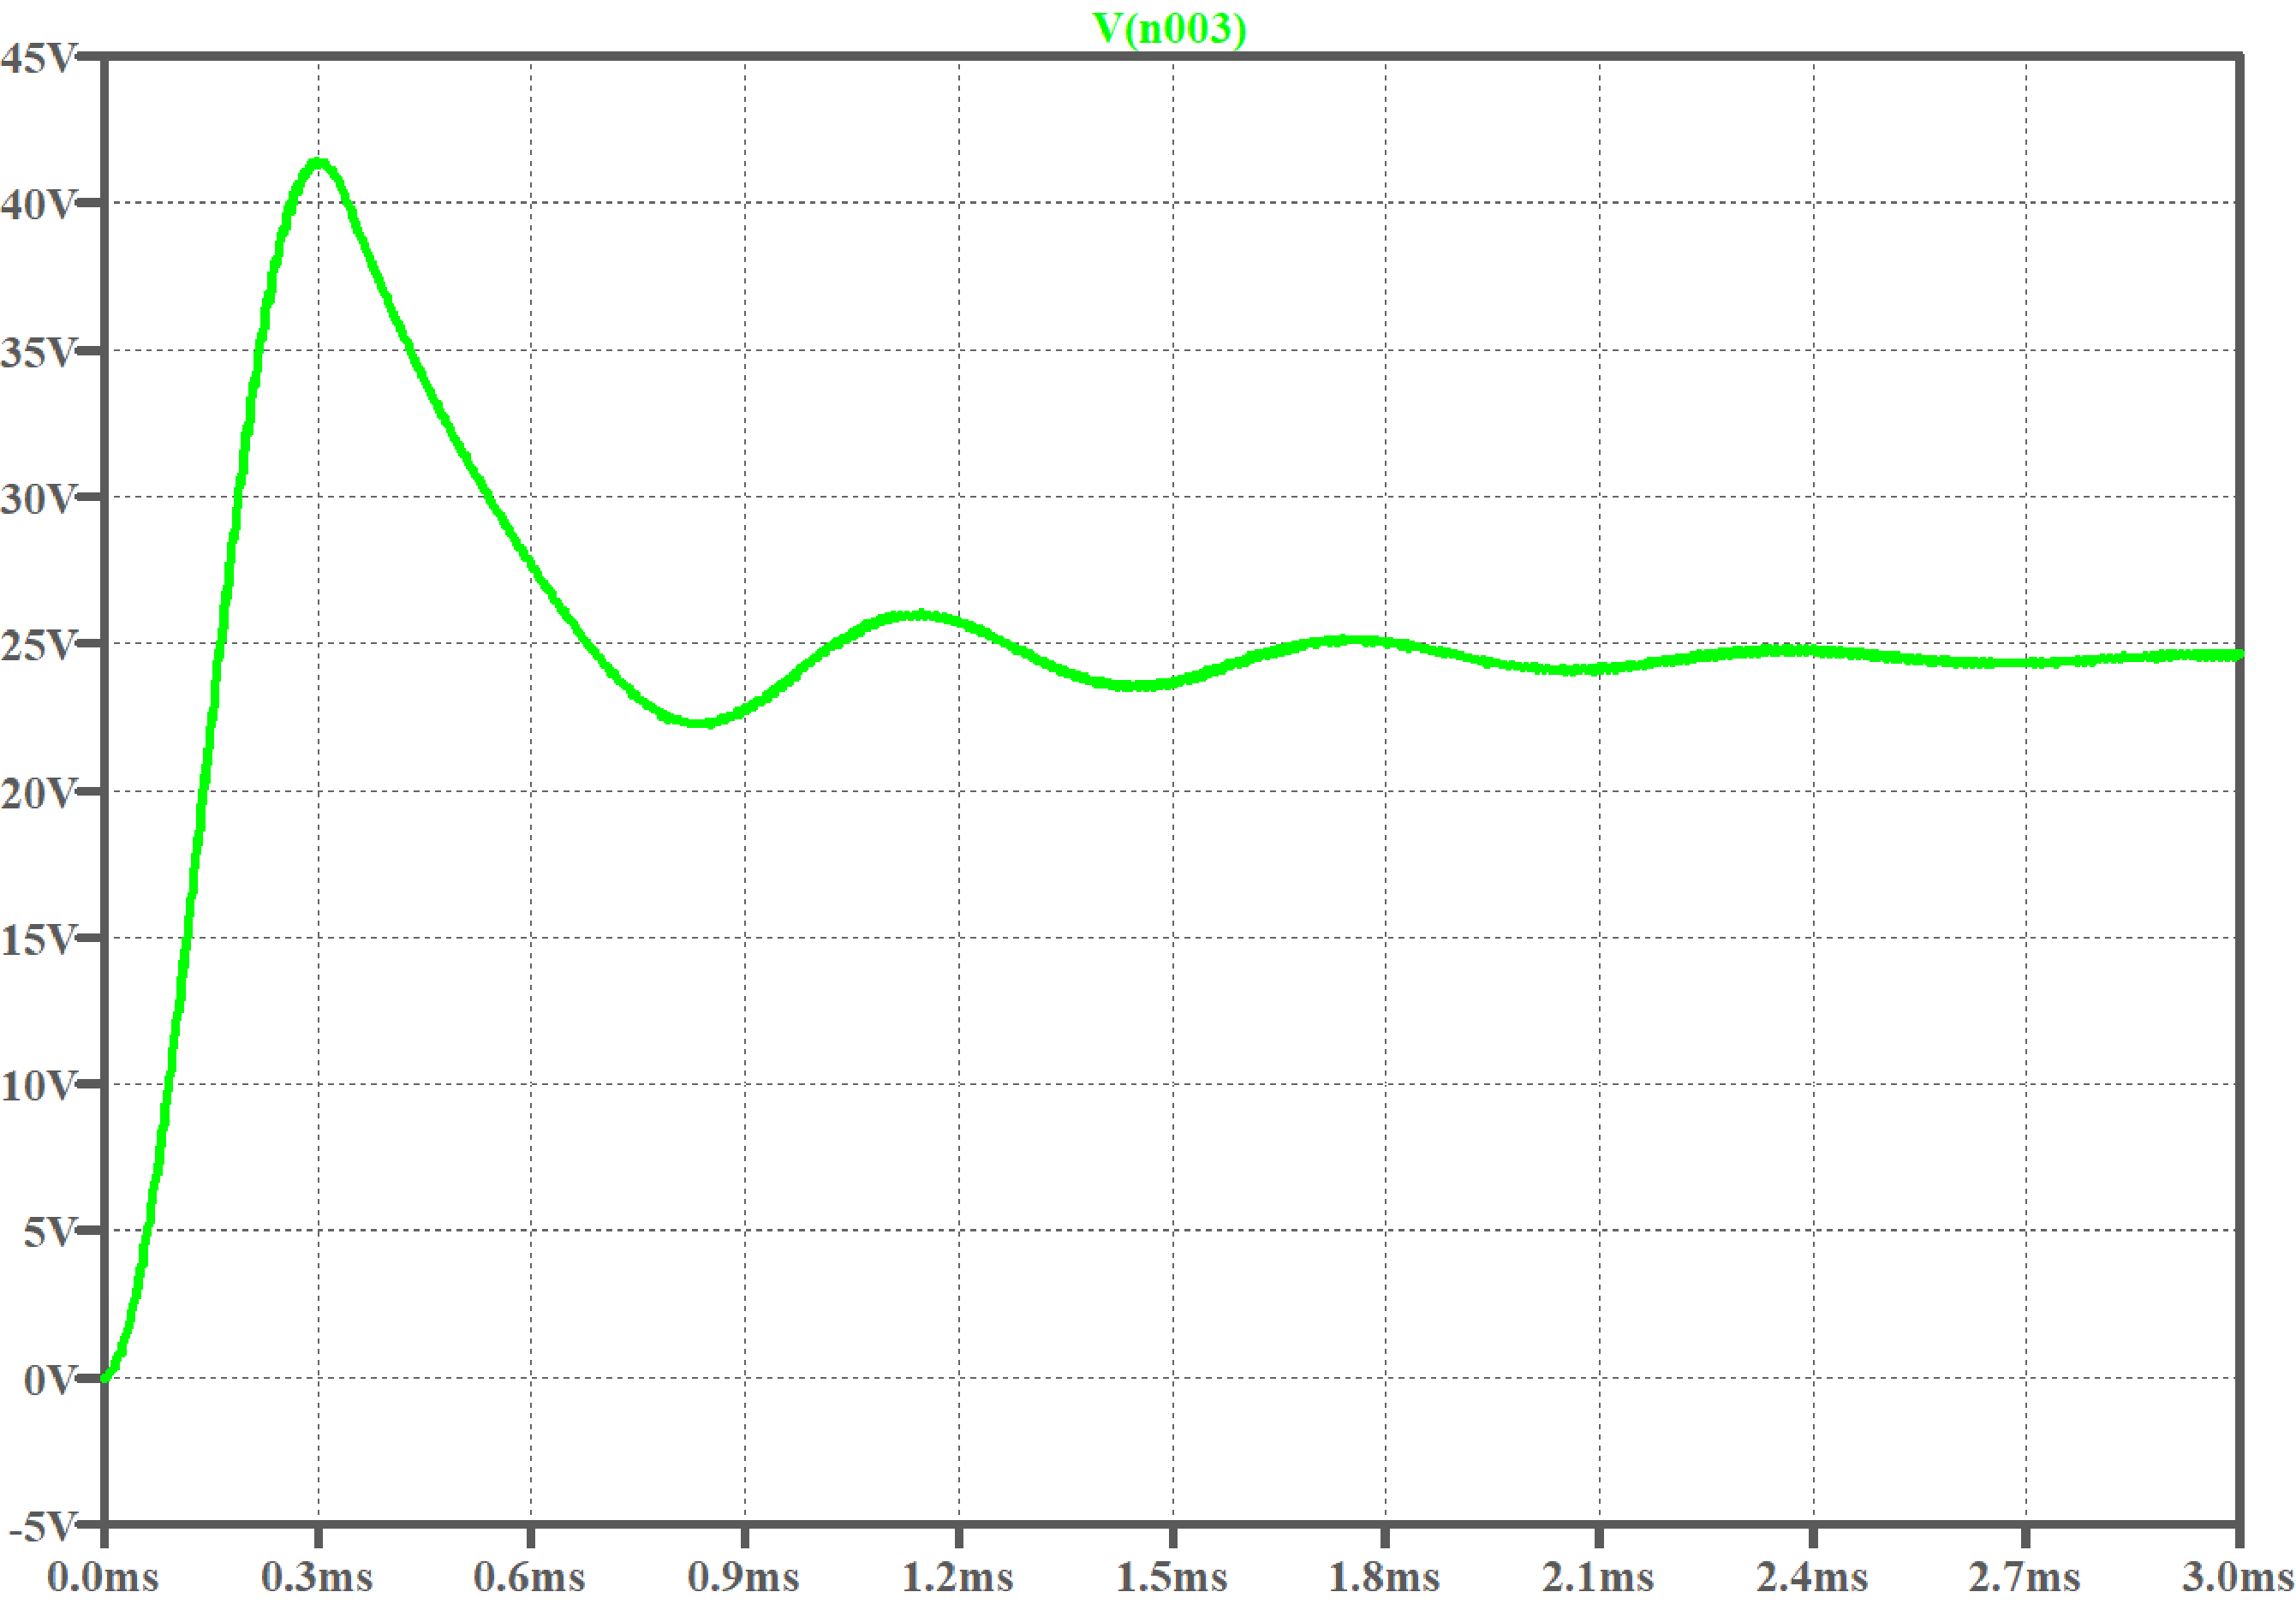
\includegraphics[width=0.55\linewidth]{Pictures/pics/LT_output_voltage.pdf}
    \caption{\textcolor{blue}{\textit{\footnotesize Flyback Converter Output Voltage Wave Form}}}
\end{figure}
\begin{figure}[h!]
    \centering
    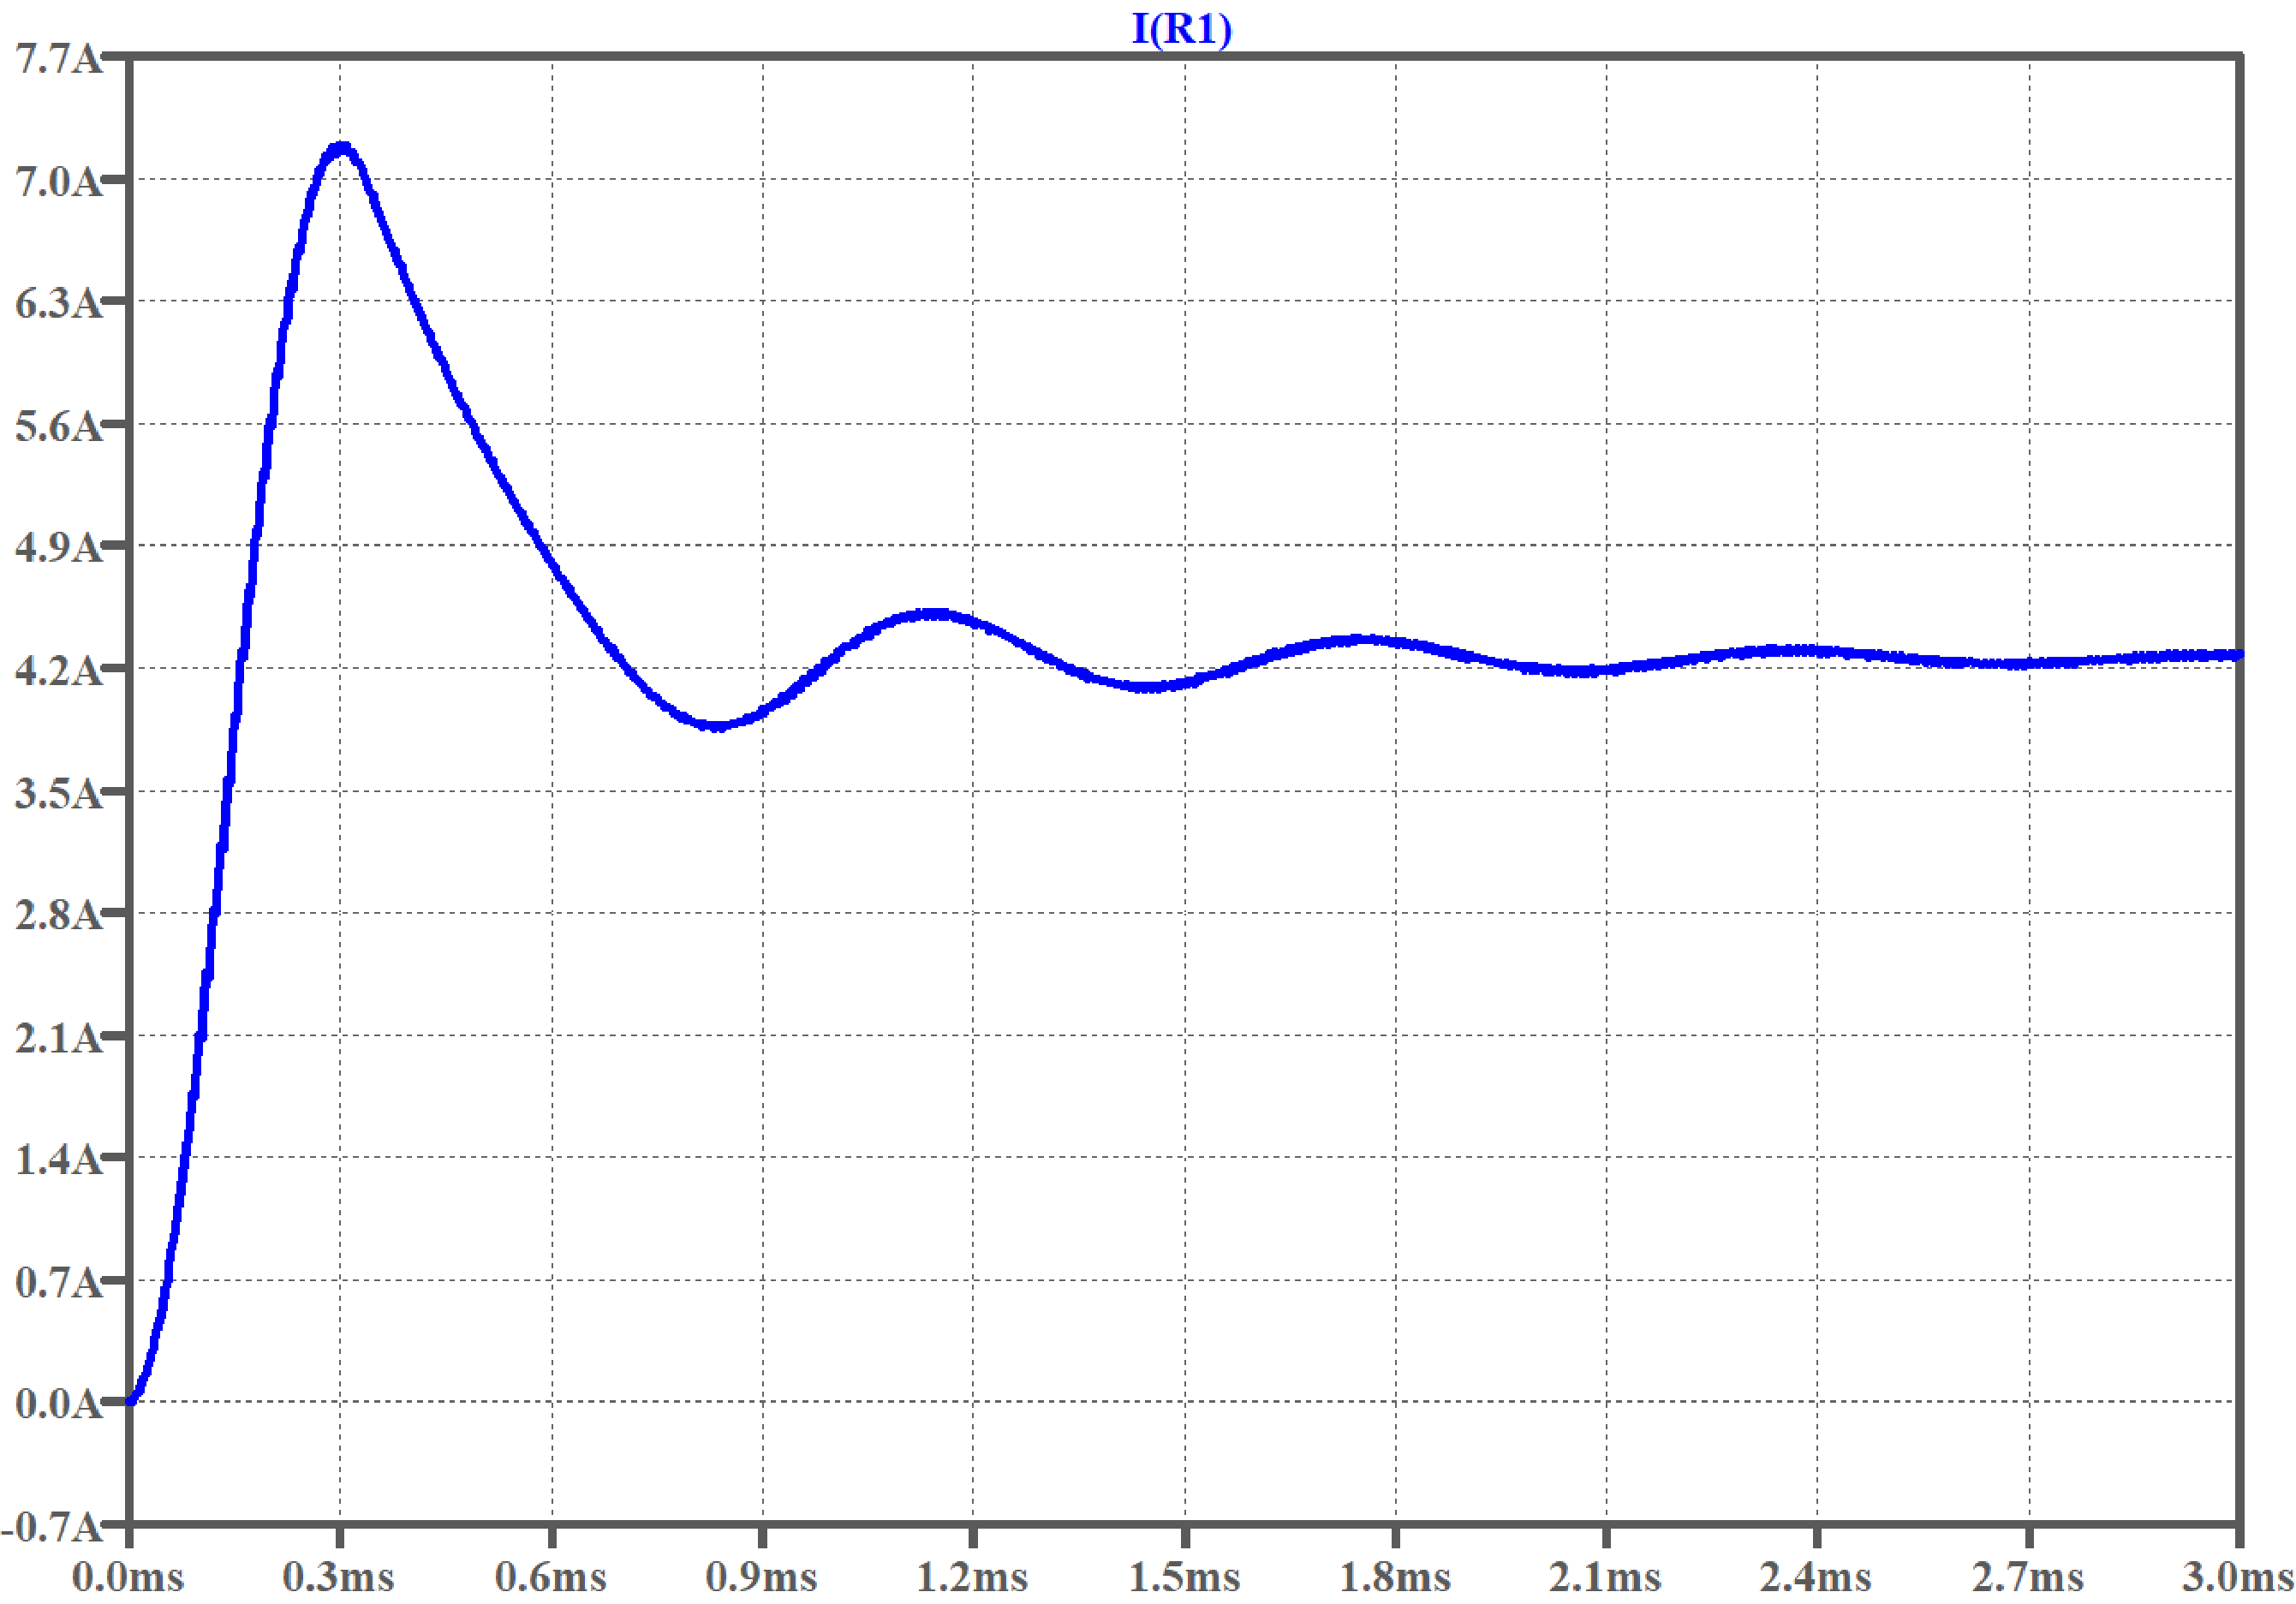
\includegraphics[width=0.55\linewidth]{Pictures/pics/LT_output_current.pdf}
    \caption{\textcolor{blue}{\textit{\footnotesize Flyback Converter Output Voltage Wave Form}}}
\end{figure}
\begin{figure}[h!]
    \centering
    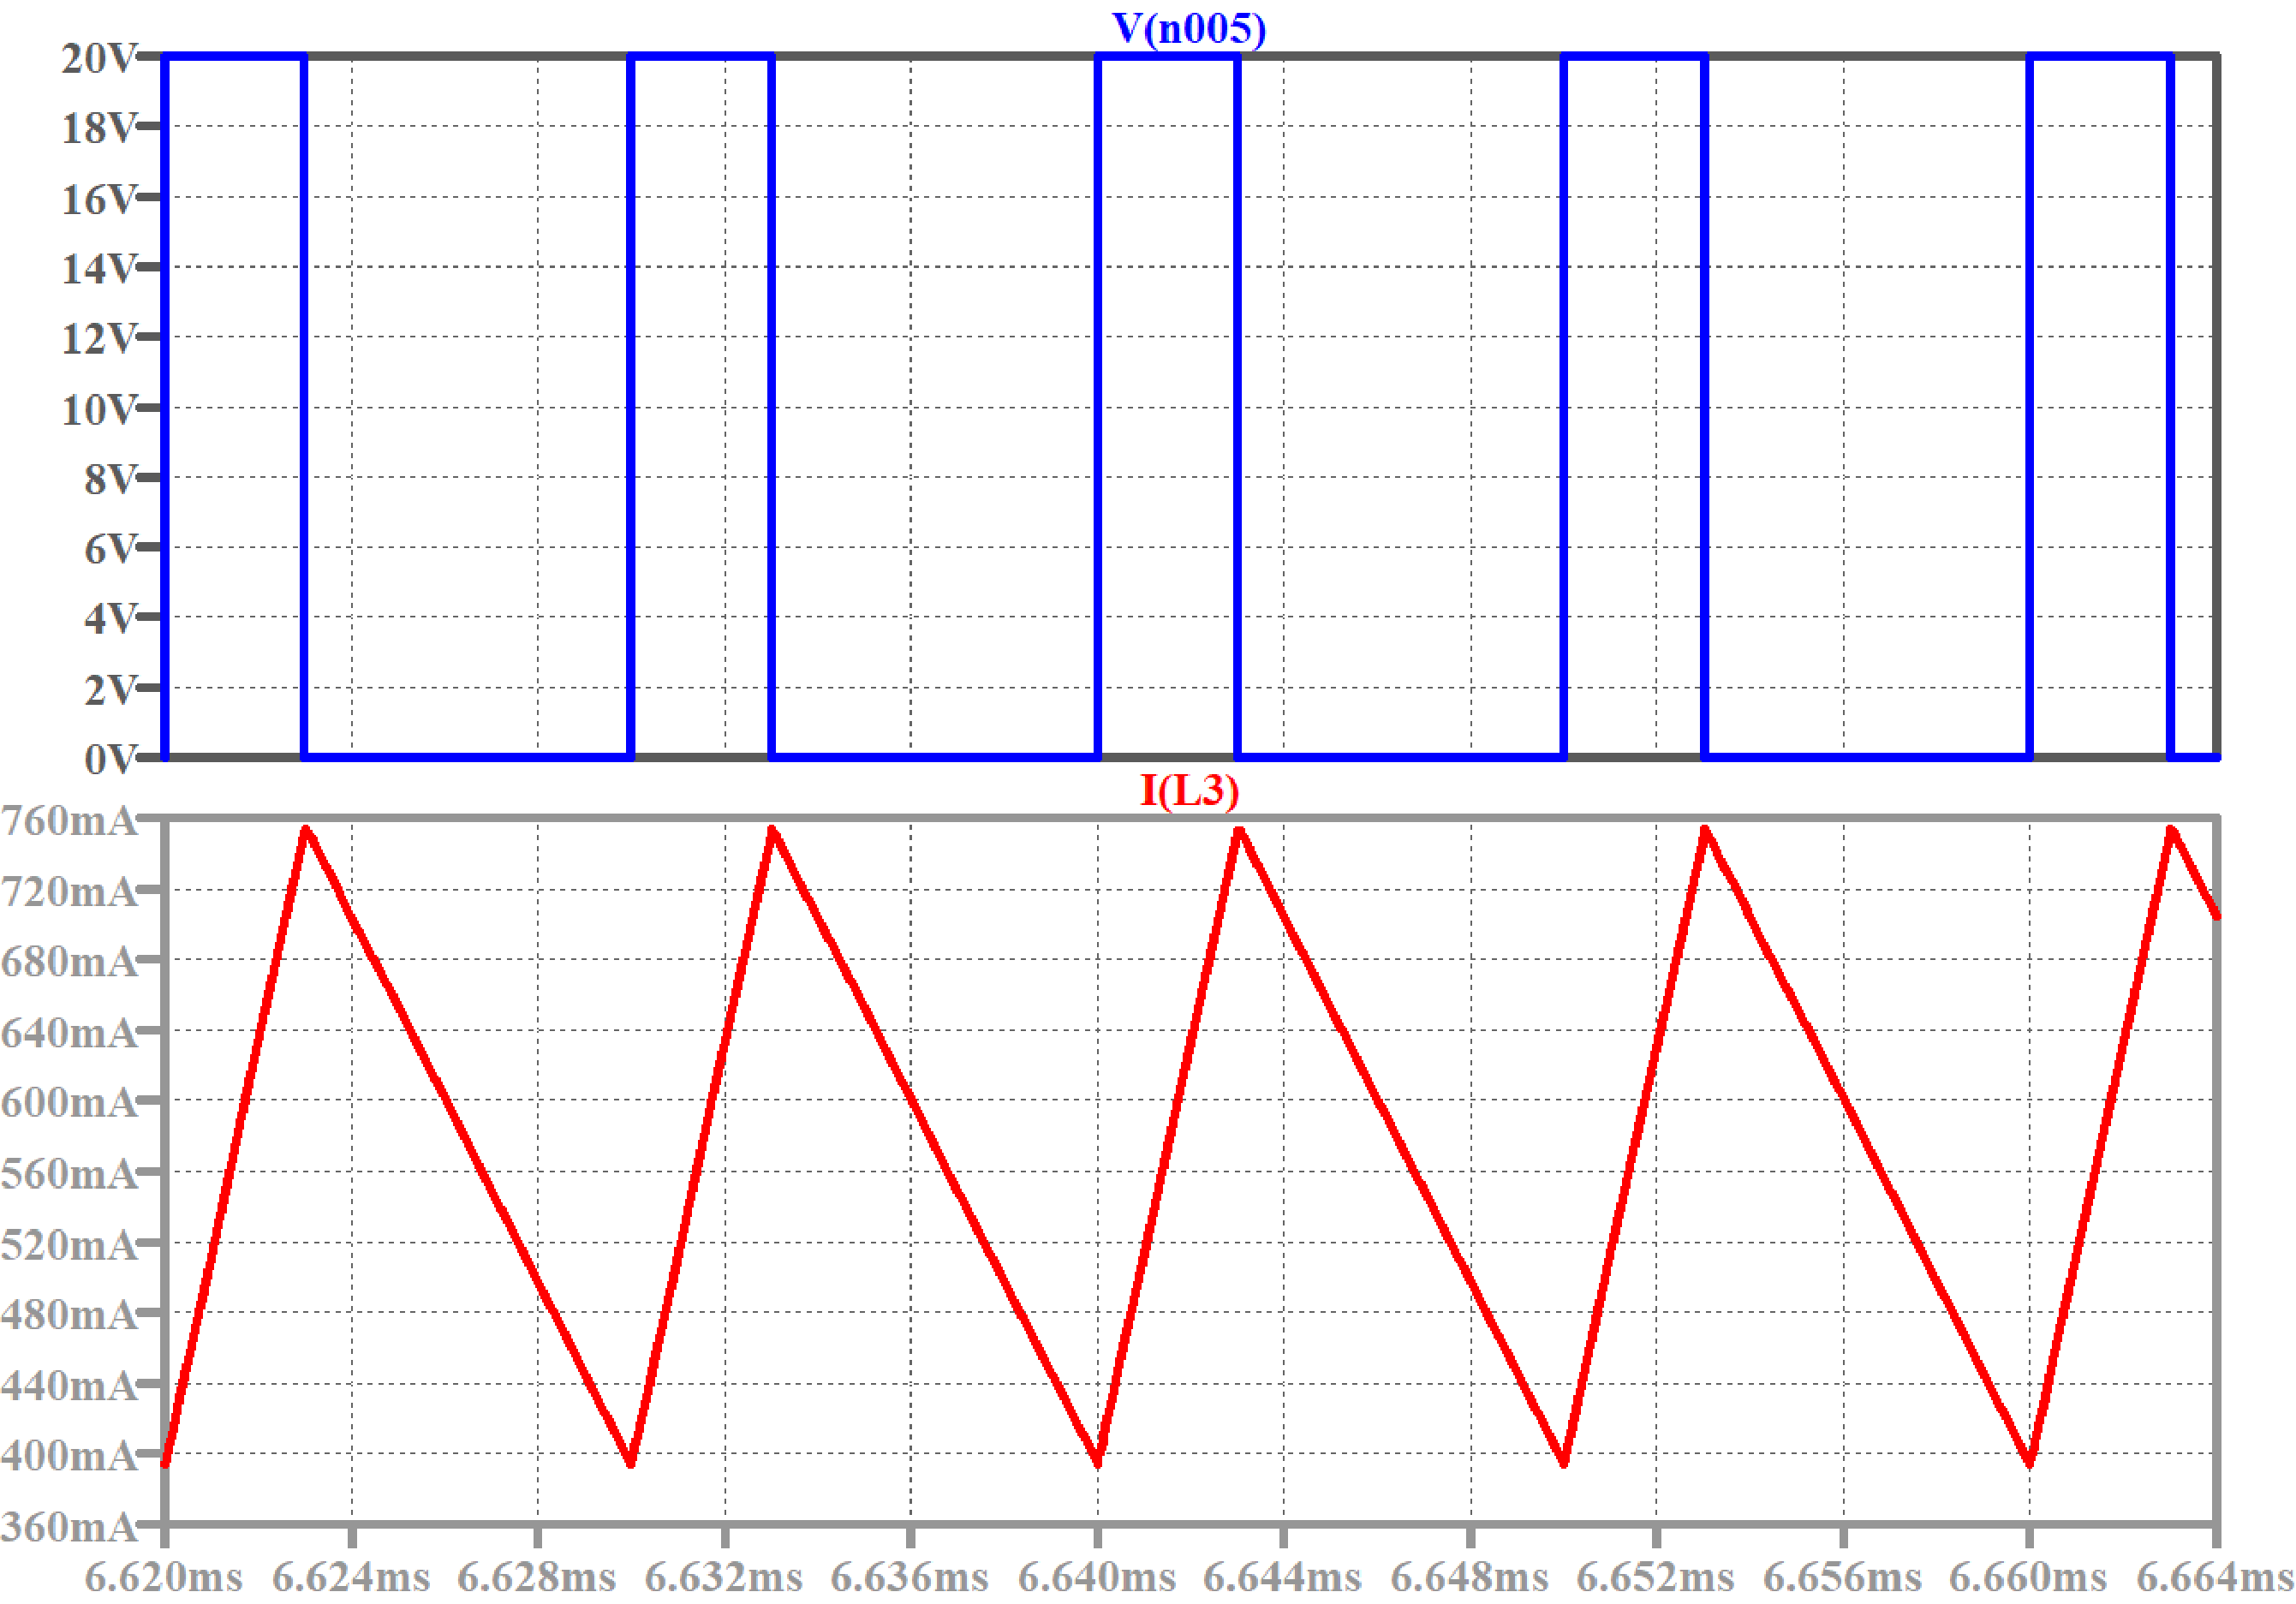
\includegraphics[width=0.7\linewidth]{Pictures/pics/L_inductance_current.pdf}
    \caption{\textcolor{blue}{\textit{\footnotesize Flyback Converter Output Voltage Wave Form}}}
\end{figure}
\end{document}
